\documentclass[12pt,fleqn]{article}
\usepackage{
  amsmath,
  hyperref,
  booktabs,
  geometry,
  graphicx,
  microtype,
  parskip,
}
\usepackage[shortlabels]{enumitem}

\geometry{margin=3cm}

% equation line spacing
\setlength{\jot}{0.5cm}

% meta data
\newcommand{\authorname}{Amo DelBello}
\newcommand{\classdescription}{MATH 1350-D2}
\newcommand{\classname}{Introduction to Statistics, Fall 2022}
\newcommand{\assignment}{Final Exam}

\newcommand{\problem}[1]{\vspace{5ex}\section*{Problem \##1}}
\newcommand{\thead}[1]{\textnormal{\textbf{#1}}}
\newcommand{\tvspace}{\vspace{.25cm}}

\title{\classdescription\ \\ \classname\ \\ $\ $ \\ \assignment}
\author{\authorname}
\date{\today}


\begin{document}
\maketitle

\problem{1}
C

\problem{2}
D \-- cannot be greater than zero

\problem{3}
Her sample is not representative of the population. The sample only contains members of a college and will probably not accurately reflect the habits of all adults in the United States.

\problem{4}
Interval \-- Differences are meaningful, but there is no natural zero starting point and ratios are meaningless


\problem{5}
D


- Null \& alternative hypotheses
- test statistic
- critical values or P-value
- state final conclusion that addresses the original claim

\problem{6}
\begin{enumerate}[label=\alph*.]
\item $H_0: \mu = 14 \text{oz.}$, $H_1: \mu \ne 14 \text{oz.}$
\item Test Statistic, t: 0.408
\item P-Value: 0.695
  \item Because the P-value of 0.695 is greater than the significance level of $\alpha = 0.01$, we fail to reject the null hypothesis. We cannot reject the claim that the mean weight of the cereal in the company's packets is 14 oz.

\end{enumerate}


\problem{7}
B \-- 0.25


\problem{8}
B


\problem{9}
As the correlation coefficient is close to zero we cannot conclude that there is any relation between the two statistics.


\problem{10}
The dice results displayed in the Actual Sum of the Two Dice histogram do not have a normal distribution.


\problem{11}
As the scores in the normal quartile plot roughly follow a straight line, we can conclude that the distribution of the test scores are roughly normal.


\problem{12}
As the P-Value for a two-tailed test is below the significance level of $\alpha = 0.04$ we reject the null hypothesis and conclude there is sufficient evidence to support the claim that the treatment group comes from a population with a mean that is different from the mean for the placebo population.


\problem{13}
A good method for determining if a data point is an influential point is to first graph the regression line resulting from the data with the point included, then graph the regression line resulting from the data with the point excluded. If the regression line changes by a considerable amount, the point is influential.


\problem{14}
A relative frequency distribution would be better in this case because it would be easier to see relationships between the two different groups, since the sample sizes differ significantly. A relative frequency distribution allows us to compare the two groups using percentages instead of the number of occurrences.


\problem{15}
The 34\% is a statistic since it applies to a sample of 1200 students, not the whole population.


\problem{16}
D


\problem{17}
Using the provided data and StatDisk, we determine the P-Value to be 0.07252. As the P-Value is greater than the significance level of $\alpha = 0.01$, we fail to reject the null hypothesis, and cannot support the claim that the treatment group is from a population with a smaller mean than the control group.


\problem{18}
B \-- $\frac{59}{80} * 100 = 0.7375$, rounded = 74\%


\problem{19}
D
\begin{align*}
  \sigma^2 &= \frac{\Sigma{(x_i - \bar{x})}^2}{N} \\
  \sigma^2 &= \frac{\Sigma{[{(5 - 9)}^2 + {(3 - 9)}^2 + {(16 - 9)}^2 + {(1 - 9)}^2 + {(20 - 9)}^2]}}{5} \\
  \sigma^2 &= \frac{286}{5} \\
  \sigma^2 &= 57.2
\end{align*}


\problem{20}
D
\begin{align*}
  \hat{p} &= \frac{316}{445} \\
  \hat{p} &= 0.710
\end{align*}

\problem{21}
C \-- The r value is outside of the values specified in table A-5 for a sample size of 6, so we use the mean as the best predicted value.

\pagebreak
\problem{22}
\begin{figure}[ht]
  \centering
  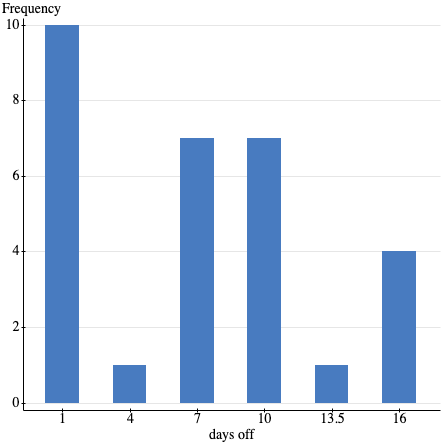
\includegraphics[width=12cm]{assets/police-days-off.png}
\end{figure}
The result does not appear to be a normal distribution because it is not, roughly or otherwise, a bell shape.


\problem{23}
B \-- Dependent samples


\problem{24}
A \-- All teachers have a one in ten chance of being selected but not every possible sample of the same size has the same chance of being chosen.


\problem{25}
B \-- 100


\problem{26}
A \-- All values are identical


\problem{27}
B
\begin{align*}
  \sigma &= \sqrt{npq} \\
  \sigma &= \sqrt{(1680)(0.57)(0.43)} \\
  \sigma &= 20.29
\end{align*}


\problem{28}
D \-- Systematic


\problem{29}
C \-- My results were slightly different. Not sure if I did it wrong? $7.95 < \mu < 11.01$.


\problem{30}
C \-- $\hat{y} = 5.05 + 1.91x$


\problem{31}
A \-- Reject the null hypothesis since the p-value is less than the significance level.


\problem{32}
D \-- 8.6 cousins
\begin{align*}
  \bar{x} &= \frac{15 + 12 + 5 + 14 + 4 + 4 + 6}{7} \\
  \bar{x} &= 8.571
\end{align*}


\problem{33}
B \-- 25.5 yr


\problem{34}
D \-- 2.8; unusual
\begin{align*}
  z &= \frac{x - \mu}{\sigma} \\
  z &= \frac{224 - 158}{23.5} \\
  z &= 2.81
\end{align*}


\problem{35}
D


\end{document}
